\subsubsection{Implementation}

Only a small change to the calling code of the fft, as well as the way the recursive calls are made is needed to adapt the recursive implementation to use OpenMP.

\textbf{Calling Code:}
\begin{lstlisting}
  #pragma omp parallel shared(timeUsed, in, out, len)
  {
    #pragma omp single
    {
      fft(in, out, len);
    }
  }
\end{lstlisting}

\textbf{Recursive Calls:}
\begin{lstlisting}
  #pragma omp task final(((len/2)/step) < 1024)
  {fft_help(dc2, dc1, len, step*2);}
  #pragma omp task final(((len/2)/step) < 1024)
  {fft_help(dc2+step, dc1+step, len, step*2);}
  #pragma omp taskwait
\end{lstlisting}

\textbf{Description of \#pragma statements}
\begin{lstlisting}
#pragma omp parallel shared(timeUsed, in, out, len)
\end{lstlisting}
Defines a parallel section which will be executed by all existing threads and tells OpenMP that the variables timeUsed, in, out and len should be shared amongst all threads.

\begin{lstlisting}
#pragma omp single
\end{lstlisting}
Defines a section which will only be executed by a single thread. This ensures that only one thread executes the recursive calls and creates the tasks. Otherwise the same task will be created by multiple threads.

\begin{lstlisting}
#pragma omp task final(((len/2)/step) < 1024)
\end{lstlisting}
Defines a task, which will be put into a taskpool where it is available for execution by another thread. If the condition in the final clause evaluates to true,
this task, and all further tasks created by it, will be executed immediately by the encountering thread. This reduces the overhead of putting the task into the pool.

\pagebreak
\begin{lstlisting}
#pragma omp taskwait
\end{lstlisting}
Tells OpenMP to wait here until the two tasks created above are completed. This is needed to ensure the correct order of execution for the Fast Fourier Transform.

\subsubsection{Performance}

Average speedup:

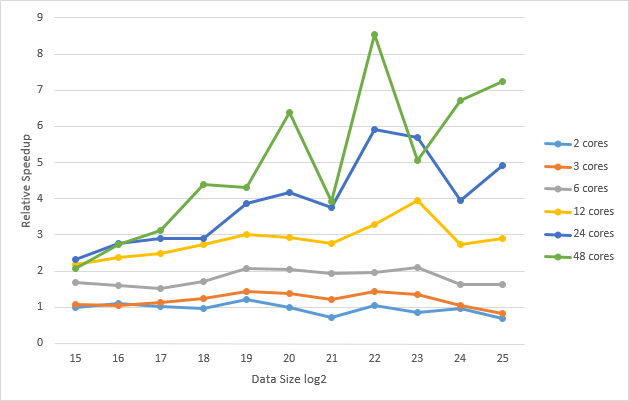
\includegraphics[width=\textwidth]{omp_rec_avg.png}

\pagebreak
Best observered speedup:

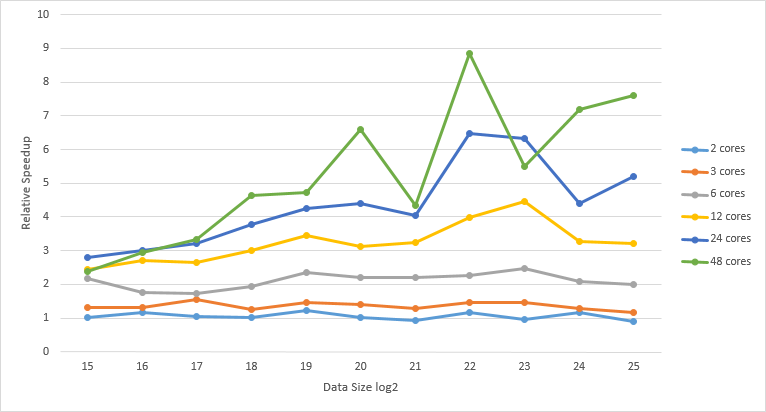
\includegraphics[width=\textwidth]{omp_rec_best.png}

What we can see here is that the speedup for larger amount of cores depends especially on the amount of data supplied.
The greater the amount of data supplied to the algorithm, the greater the amount of tasks created by the program. Further down the recursion tree this leads to the creation of
a large number of tasks, for which there is very little to compute. This would lead to a slowdown because of the overhead associated with switching threads and assigning tasks to threads.
We tried to mitigate this effect by introducing the cutoff value. 1024 was chosen as the value, that delivered the best results during testing. Larger cutoff values led to higher amounts of computation to be done and thus lower speedups overall.
But even with this cutoff there is a drop in speedup after \(2^{23}\) which seems to be the point at which the thread scheduling overhead takes over again.

Another (and probably the largest) factor that limits the speedup is memory access time. The data accesses in the FFT algorithm are all spaced fairly far apart, which causes elements that are needed in a task to be stored so far apart in memory,
that they will be put into different cache lines. This in turn leads to more lines being fetched from memory, as well as more cache misses.
